\chapter{Methodology}~\label{chapter-methodology}
\epigraph{Is there method in the madness?}{Anon (1964--on)}
\buzzwords{Empirical Studies, Theoretical Framework, Conceptual Framework, make assumptions explicit, methodological analysis using prior publications to identify a vocabulary - SE in practice, qualitative analysis,  the 1-2-3 of research design (question - evidence - method) ...}


\begin{wrapfigure}{R}{0.7\textwidth}
  \vspace{-0.75\intextsep}
  \begin{center}
    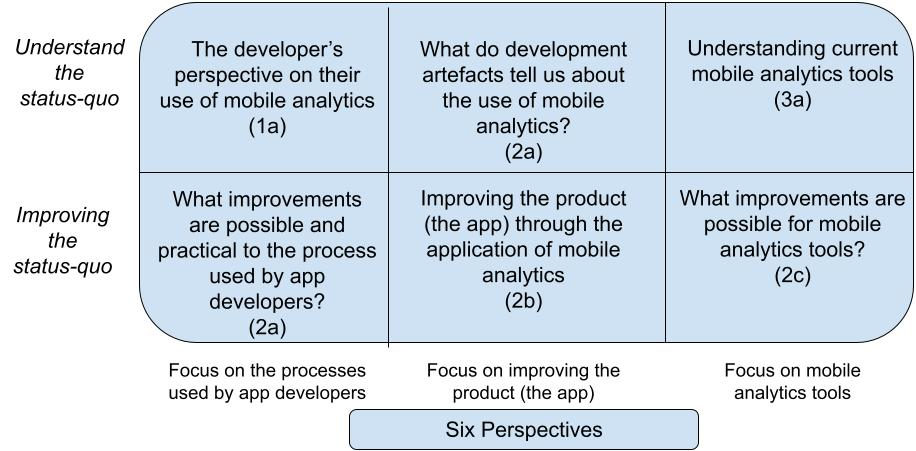
\includegraphics[width=0.66\textwidth]{images/my/six-perspectives-2x3-matrix-25-oct-2021abc.jpeg}
  \end{center}
    \caption{Methodology six perspectives (repeated)}
    \label{fig:six-perspectives-in-the-methodology}
\end{wrapfigure}

To answer the research questions there needs to be evidence from how developers use mobile analytics in practice, therefore the methodology needs to include techniques that focus on practical aspects of app development, the use of mobile analytics tools by these app development teams, the quality of these tools, and consider the value and impact from the perspective of these teams.

The data needs to be rich and from real-world apps and projects which justify the use of cases. The research also had to engage with Industry and take a case-based approach situated in real projects. 

\newthought{The research needs to be situated in the real-world}
As the real-world apps live in an app-store ecosystem and as the main app stores collect app analytics the research needs to be situated in apps that are available in an app store. And as the analytics are derived from usage the apps need to be used, ideally by real-world users of those apps. A variety of projects and apps may help to uncover emergent features, capabilities, and behaviours; they may also help to establish a range of examples of any improvements and any concerns. 

No two analytics tools are identical, they offer a variety of features, capabilities, and have distinct behaviours. Developers use a variety of these tools, therefore there is value in researching various mobile analytics tools. Furthermore there are tools that work at the platform level and others that work at the app level, again researching tools that work at both levels helps determine and distinguish their characteristics and compare their behaviours. 

Interim actions:
\begin{enumerate}
    \itemsep0em
    \item Map the methods to the six perspectives in Figure~\ref{fig:six-perspectives-in-the-methodology}. 
    \item Mapping of perspectives into the data that drives them - justify the evidence that each perspective would need.
    \item Data collection methods that will deliver the evidence: I now have the foundation for the rich data I want to collect.
\end{enumerate}

% Data needed - justify the use of cases
% Therefore...
% Data I am seeking
% Map the data onto the analysis

\begin{table}
    \small
    \setlength{\tabcolsep}{4pt} %% default is 6pt
    \setlength{\arrayrulewidth}{0.1mm}
    \centering
    \begin{tabular}{l|ccc|ccc}
      & \multicolumn{3}{c}{\bfseries \small Understand} & \multicolumn{3}{c}{\bfseries \small Improve} \\
      \toprule
         % &\textsubscript{u}Use &\textsubscript{u}Artefacts &\textsubscript{u}Tools &\textsubscript{i}Use &\textsubscript{i}Artefacts &\textsubscript{i}Tools \\
         &U\textsuperscript{use} &U\textsuperscript{artefacts} &U\textsuperscript{tools} &I\textsuperscript{use} &I\textsuperscript{app} &I\textsuperscript{tools} \\
         
        \hline 
        \textbf{Sense-making} & & & & & & \\
        Beacon finding and    &Y &y &Y &y &y &y \\
        Drill Down            &y &y &Y &Y &y &y \\
        \tabucline[1pt on 3pt]  \\ % See https://tex.stackexchange.com/a/109301/88466 however here it is terminated prematurely and a bit heavy 
        % Or try https://tex.stackexchange.com/a/229334/88466 or https://tex.stackexchange.com/a/613907/88466 if I've not collapsed these two previous rows soon.
        % Or use a newer latex package, see https://tex.stackexchange.com/a/611494/88466 
        Local App Experiments &y &Y &Y &  &Y &Y \\
        
        \hline
        \textbf{Evaluation through action research} & & & & & & \\
        Field Experiment      &y &  &  &Y &Y &  \\
        Embedded              &y &Y &y &Y &Y &y \\
        Hackathon             &y &y &  &Y &Y &  \\
        
        \hline
        \textbf{Feedback mechanisms} & & & & & & \\
        Ask The App Devs      &Y &y &y &y &y &  \\
        Ask The Tool Devs     &  &  &Y &y &y &y \\
        Grey Literature       &y &y &Y &y &y &  \\
        Code Analysis         &y &Y &  &y &  &  \\
        
        \hline
        \textbf{Across case comparisons}            &Y &y &Y &Y &y &y \\
        \bottomrule
    \end{tabular}
    \caption{Mapping Research Methods to the 6 perspectives}
    \label{tab:mapping-analysis-to-six-perspectives}
\end{table}


\begin{figure}
    \centering
    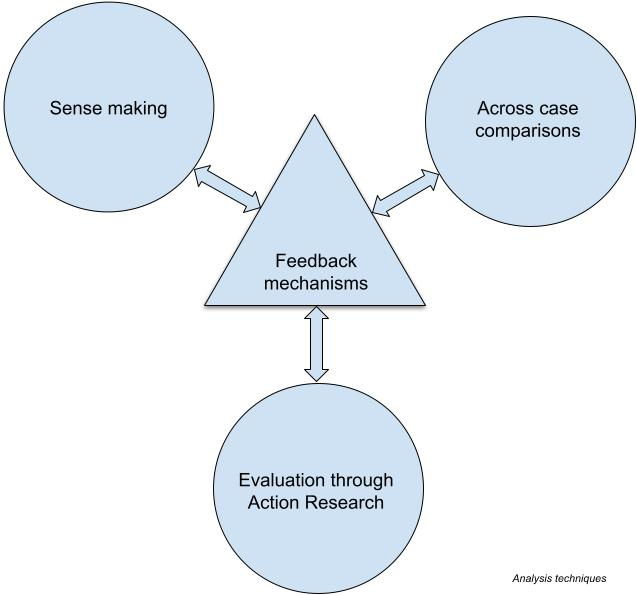
\includegraphics[width=12cm]{images/my/analysis-techniques-in-PhD-25-Oct-2021.jpeg}
    \caption{Analysis techniques illustrated}
    \label{fig:analysis-techniques-in-phd}
\end{figure}

\section{Overview of the research methods}
\julian{This is as much to help ensure I understand the methods and communicate them adequately to you. I expect this section to be heavily revised before submission.}
Each of these research methods includes data collection \textit{and} analysis unless otherwise stated. Some include several data sources and some data sources are analysed using several methods. The methods and the data sources often also inform several of the six perspectives.


Figure~\ref{fig:analysis-techniques-in-phd} provides a visual overview of the four categories of analysis techniques; They include sense-making, evaluation through action research, and comparisons across cases. Various feedback mechanisms help to support and validate the rest of the analysis techniques. 


\subsection{Sense-making}
% c.f. https://en.wikipedia.org/wiki/Sensemaking_(information_science)
The following methods primarily helped with sense-making: analysing and ``making sense" of mobile analytics tools, development artefacts, and the developers' perspectives on their use of mobile analytics. 

TODO discuss the work of~\citep{naumer2008_sense_making}

\subsubsection{Beacon-finding and drill-down}
\textbf{Beacon finding} seeks for potentially relevant indicators, typically within bounded domain. In this research the domain may include: a mobile analytics report, a method call in source code, a developer's description of their use of mobile analytics to assess the quality of the app, and so on. Beacons help to convey meaning and are used for comprehension, for instance by programmers who wish to understand source code~\citep[page i]{crosby2002_roles_beacons_play_in_comprehension_etc}.

\begin{comment}
Commented out after adding the grouping suggested with Marian on \nth{22} Oct 2021. Preserved until this chapter is in better shape.

\julian{Conflations: 1) data collection methods and analysis 2) contributors and goals also conflated. Action: Group rows by what I was targeting: I need to provide the rationale for the methods I used.} Two suggested groupings to try:
\begin{itemize}
    \item 3 Groupings: Tool outputs, validation, action research. 
    \item 4 Groupings: beacons-and-drill-downs, comparisons, contextualisation and clarification, evaluation through action research.
\end{itemize}
\end{comment}


Usage can be generated by actual users, emulated by other people, simulated by automated scripts interacting with apps, generated by programs, and fabricated by providers of mobile analytics tools/services. Of these, usage generated by actual users is inherently part of the real-world microcosm developers of the apps inhabit and therefore the research methods need to understand the use of mobile analytics in this context. 

There may be various ways to access the real world data, such as being a part of the development team, or being granted access by the development team. While the providers of the mobile analytics services may also have access various ethical, commercial, non-disclosure, safeguarding, and additional considerations make such access unlikely even though it could be tremendously rich and insightful. Some of the research can be performed using emulators and/or simulators and allows for greater control of the input conditions.

\dotfill

Need to understand what data is actually available that I can collect.
From data to analyses I am undertaking.
In order to get this data 

Therefore I'm going to have to engage with Industry. A case approach, situated in real projects.
How can we generate the evidence and what data can we collect to partially answer the demands for evidence. c.f. data sources section. Provide a foreshadowing of the data sources, signpost to where they will be discussed.

Instantiation in the introduction to the case studies chapter after the model described in the methodology.
Move 5.1 into the methods chapter as it provides orientation for the reader.

I need to decide on my primary organising principle: e.g. the 6 perspectives
Rewrite section 5.1 around figure 5.2 (6 perspectives) Label the 6 perspectives.

In order to understand .... this is what we need, therefore we use the following methods to gather the evidence.

DevEx of the use of the mobile analytics. 

Create a table of the needs to fulfil each of the 6 perspectives: data needed to perspectives i.e. purpose of Analysis, framed in terms of these 6 perspectives. 
Justify how each data source is used to fulfil the research questions. 

From question to evidence to method.

Once the above has been sketched out I can then discuss my roles and I was aware I take different roles and my analysis was cognisant of the different roles I played.

I'd need to define what a case study is. - an opportunity to look in depth in the real world, a container for data collection with and in a number of organisations. I'll explain clearly what methods I was able to use in each case. 

Let me explain in more detail what I mean by... 

*** P1 Start with the table for cases -> types/ categories of data 
*** P2 Table Data types mapped to the analysis I could perform on that data type. What method I used to analyse the data.
Analysis to method may be easier to generate than analysis to purpose.

\begin{figure}
    \centering
    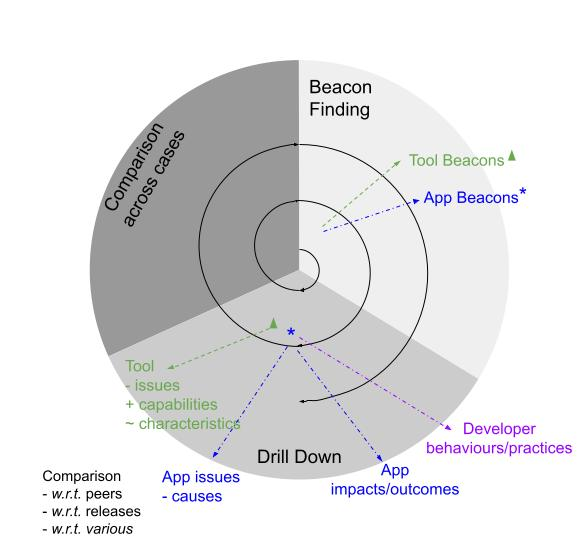
\includegraphics[width=14cm]{images/my/Illustrated-Research-Methodology-using-Mobile-Analytics-as-the-Epicentre-v0-2.jpeg}
    \caption{Illustrated Research Methodology using Mobile-Analytics as the Epicentre}
    Illustration of the 
    \label{fig:Illustrated-Research-Methodology-using-Mobile-Analytics-as-the-Epicentre}
\end{figure}

\section{Analytics centric methodology}
The methodology incorporates an iterative cycle of \textbf{beacon finding} to identify areas of interest within a case, \textbf{drill down} to investigate one or more beacons, then \textbf{comparison} across cases to identify patterns, relationships, counterfactuals~\footnote{\emph{``relating to or expressing what has not happened or is not the case." Oxford Languages.}}, as some characteristics emerge in contrasts across and between a body of studies. The first representation of the iterative cycle is illustrated in Figure~\ref{fig:Illustrated-Research-Methodology-using-Mobile-Analytics-as-the-Epicentre}. This shows an artificially clean and orderly progression between elements in the cycle and useful to communicate the concepts of the research methodology. 

However this Figure (\ref{fig:Illustrated-Research-Methodology-using-Mobile-Analytics-as-the-Epicentre}) does not incorporate real-world and practical characteristics of app development practice, which is the crucible for this research. The research needed to be grounded in real-world projects and with real-world app development teams, accordingly the methodology incorporates a mutually-beneficial, symbiotic, bi-directional connection where the iterative research is evaluated with and through these real-world projects and teams. Figure~\ref{fig:illustrated-combined-methodology} includes the bi-directional connection and also illustrates a modified progression between the elements in the iterative cycle where the iteration alternates primarily between beacon-finding and drill-down, and less frequently through the comparison element. All these elements are vital and none less important than the others. Again the figure is representative, for individual cases the flow and progression may well vary.

This Figure (\ref{fig:illustrated-combined-methodology}) also partly indicates how the research feeds the six perspectives to varying degrees; (the evaluation and action research also contribute to the six perspectives). TODO divide this figure. Create another figure to show the sources to the 6 perspectives. 

TODO Motivation for the methodology. 

Need something comparable for the messy tail of the figure. Then these can be mapped onto the 6 perspectives. 

\begin{figure}
    \centering
    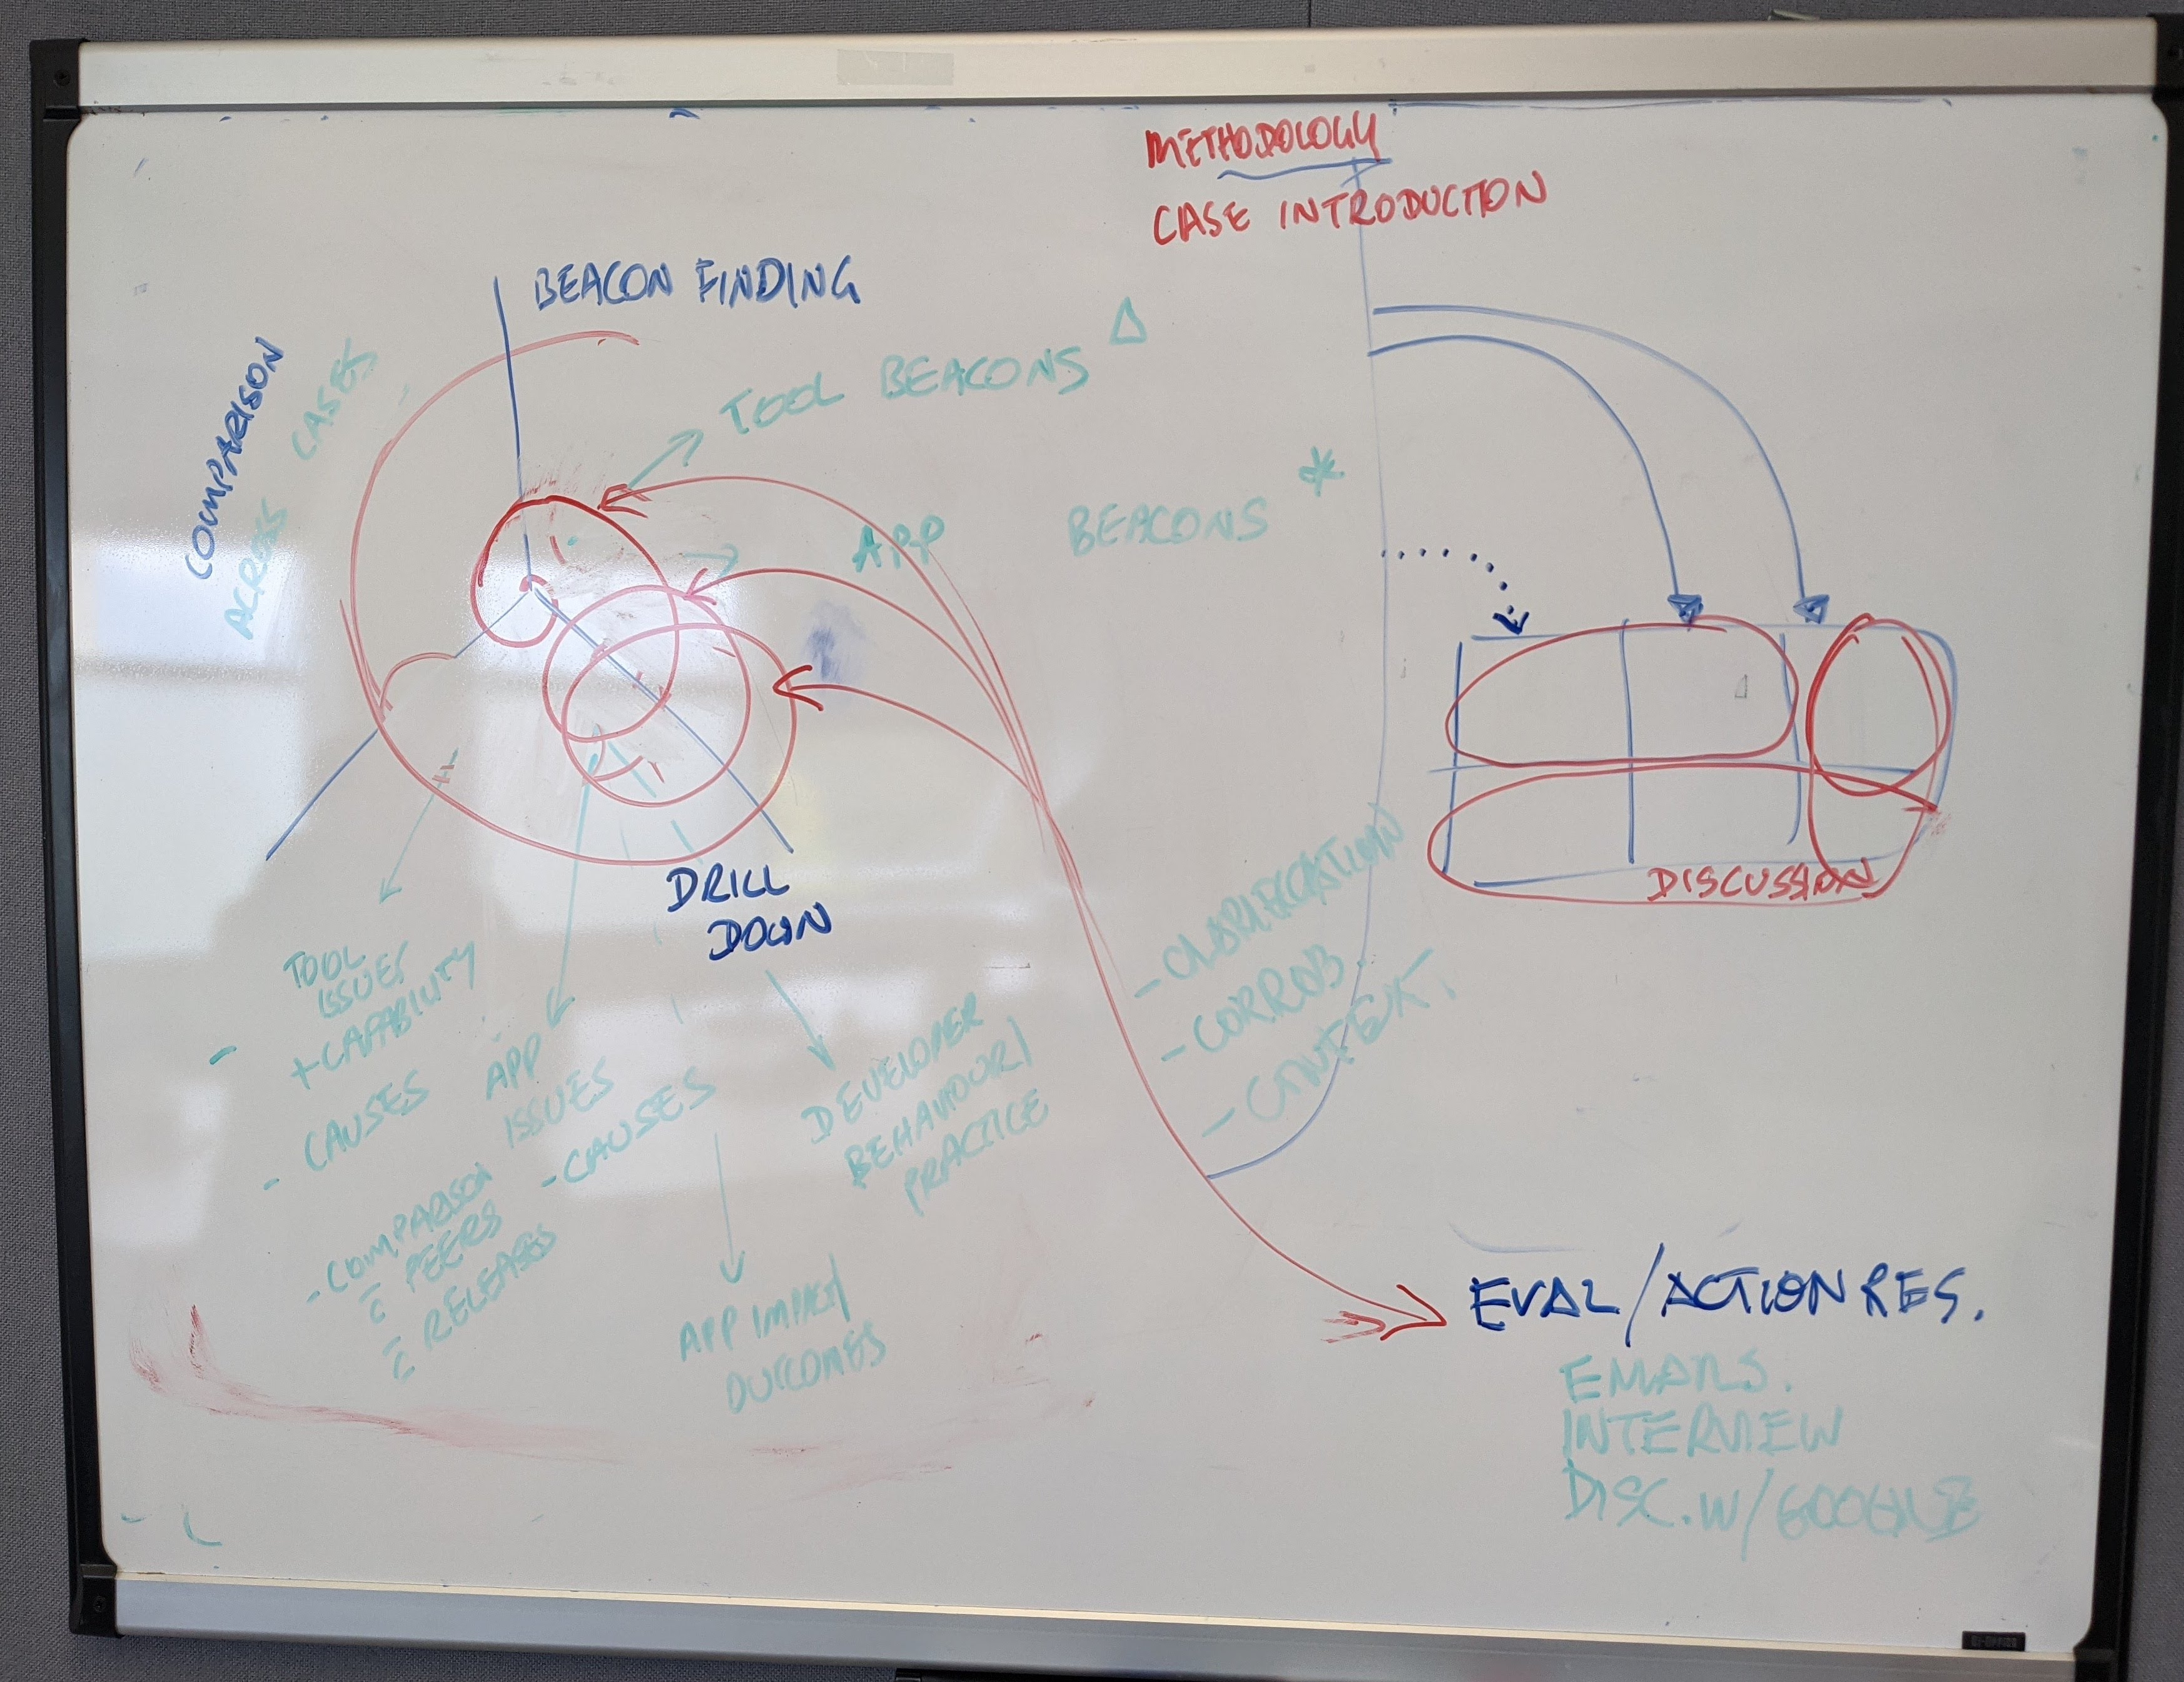
\includegraphics[width=14cm]{images/my/illustrated-combined-methodology-v0-1.jpg}
    \caption{Illustrated combined methodology}
    \label{fig:illustrated-combined-methodology}
\end{figure}

This corresponds in principle to the structure and premises of grounded theory where patterns are induced, data iterated to see if categories are appropriate, identifying patterns with comparisons with other data sets for checks and balances. 

TODO discuss saturation briefly. 

Not only could this be connected to context, it could be applied in practice to see the effects of the results.

Need to map methods to perspective. 


\section*{Preamble - what needs doing to craft this chapter}
{\small
Recap what I found in the Literature Review, to validate the RQs. Then start with the RQs to consider how they can be answered in the research. Highlight the value and relevance of evaluating this in practice. Add `in practice' to my RQ. Look at literature on the theory of generalisation from case studies - Ask Marian for advice on this.

Determine what's needed to answer each sub-question and the methods needed to answer them. Formulate hypotheses from the RQ's - consider first falsifying the null hypothesis. Pointers: the research onion - Saunders, appeals to logic, appeal to authority - prior practice, what are the threats to validity, maintain the methods developers use which is outside the scope of this chapter,

Create a diagram to map out the connections between the case studies and the evidence they provide. Show the dependencies between the RQs and the case studies and the evidence they provide.

Arosha suggested a layered diagram with evidence at the base. or perhaps something akin to Akshika's diagram~\ref{fig:akshikas-methodologies-map}.
}

\begin{figure}
    \centering
    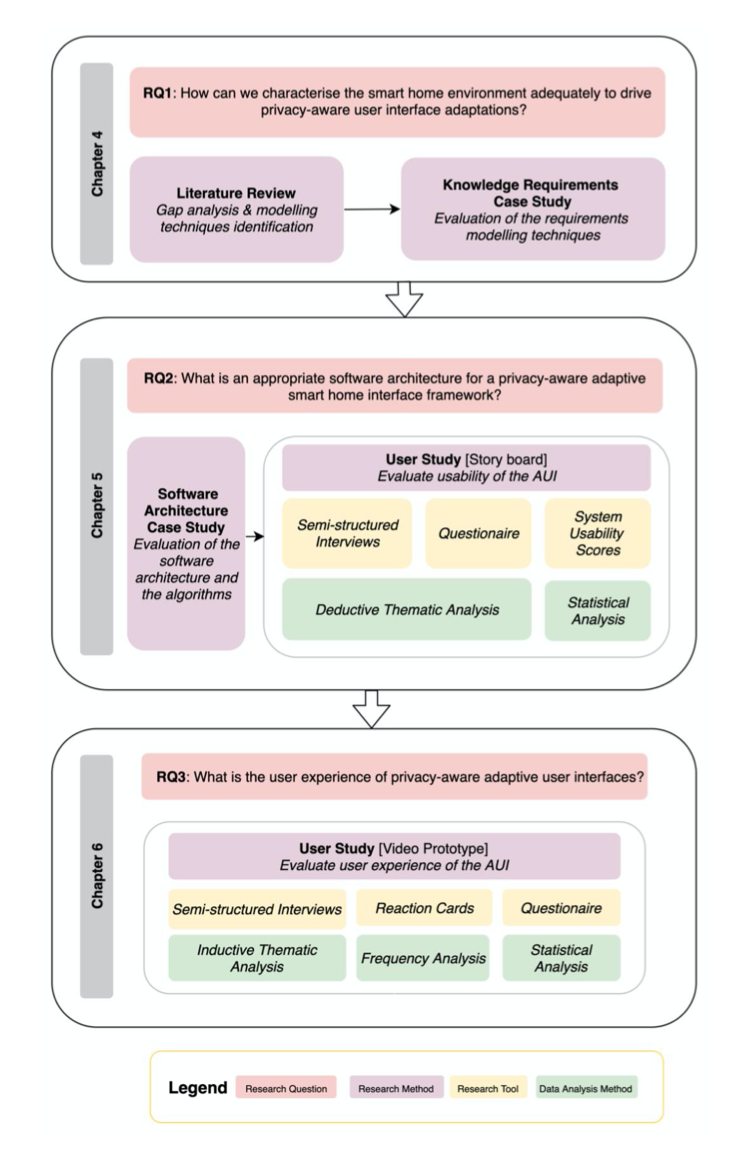
\includegraphics[width=9cm]{images/ephemeral-images-remove-pre-publication/Akshikas-methodology-diagram-from-his-thesis.png}
    \caption{For inspiration only: Akshika's methodologies map}
    \label{fig:akshikas-methodologies-map}
\end{figure}

\hrulefill
\clearpage


\section{Text-based methodology maps (a w-i-p)}
\emph{The following hierarchical lists are a work-in-progress while the details are established. They will be replaced and retired.}


{\footnotesize
\begin{description}
    \itemsep0em
    \item[Research Method] :
        \begin{itemize}
            \item Case Study
        \end{itemize}
    \item[Research Tools] :
    \begin{itemize}
        \itemsep0em
        %\item[]
        \item Action Research
        \item[$\bullet$] [Semi-] Controlled Experiment (Field experiments)
        \item Hackathon
    \end{itemize}
    \item[Analytics Provider] :
        \begin{itemize}
            \item Google Play Console with Android Vitals
        \end{itemize}
    \captionof{methodology-map}{Kiwix case study methodology map}
    \label{methodology-map-kiwix-case-study}    
\end{description}
}
% Thanks to https://fedoramagazine.org/latex-typesetting-part-1/ for helping me discover {description} and for enabling me to find workarounds when it didn't render as I'd expected e.g. where I needed to add [$\bullet$] to stop it interpreting [Semi-] as a style.

{\footnotesize
\begin{description}
    \itemsep0em
    \item[Research  Method] :
        \begin{itemize}
            \item Inductive analysis of source code
        \end{itemize}
    \item[Research Tool] TBC
    \item[Data Analysis Method] TBC
    \captionof{methodology-map}{Logging using Mobile Analytics}
    \label{methodology-map-logging-using-mobile-analytics}
\end{description}
}

The logging case study, in \secref{methodology-map-logging-using-mobile-analytics} uses inductive analysis to determine the patterns. 

\section*{Plain thoughts on the methodology used}
Methods need to support real-world projects, their development teams and their apps. Case studies enable this so they were used for the core of the research. Each case study needed the support and agreement of the project team who needed to provide access to the mobile analytics services they use. Those teams and their respective organisations had a bearing on the scope and limits of the research that would be acceptable to them, this meant that case studies were opportunistic in nature and depended on the alignment of purposes, timings, and so on.

There was a fair amount of housekeeping needed to provide and maintain access (where permitted) to the tools. Some teams also allowed access to their bug tracking systems, their source code (and associated build, CI and testing), and - of necessity - their mobile analytics reports. Some wishes aspects of their microcosm to be kept private, in some cases, representative alternatives could be provided that illustrated and/or exemplified some of the learning while maintaining their anonymity.  

Many of the case studies provided extended access to some or all of their systems which enabled some post case study analysis. Learnings from some case studies were able to be used in subsequent ones.

Even though the case studies provided really useful and relevant findings it was clear they did not represent the population of mobile apps. Various Industry contacts who actively use at least one mobile mobile analytics service to monitor failures in their apps agreed to be interviewed and share their insights. Their involvement was approved by their respective projects and/or organisations addressing combined business and ethical perspectives. Again, owing to their specific contexts, concerns, and experiences the interviews were semi-structured to enable them the flexibility, control and freedom to share whatever results, experiences, and insights they were willing and able to provide.

There were some experiments that were not sensible/practical in the case studies; so small scale experiments were designed and performed to research those when it was viable to do so. The ephemeral nature of data and reports in several of the mobile analytics services meant these data and reports were originally hard to record and preserve. The research therefore included the development of software that was able to preserve the data and reports from the core mobile analytics service: Google Play Console with Android Vitals.

Several mobile analytics providers became interested in the research and the results and their perspectives was also of interest and germane to the research, therefore there were symbiotic sharing of results, analysis, product design, customer insights and so on. All these have been anonymised by at least one party and non contained personally identifiable information.  

\newthought{Conceptual Framework}
``Conceptual frameworks provide a theoretical overview of your intended research and order withing that process", ``a map or framework of how the research will be conducted and analysed"~\citep[page 44]{trafford2008_stepping_stones_to_achieving_your_doctorate}

Germane concepts include:
\begin{itemize}
    \item Value Chains and modelling Influences, e.g. see \emph{``From Data to Decisions: A Value Chain for Big Data"}~\citep{miller2013_from_data_to_decisions_a_value_chain_for_big_data} which provides 7 stages in a value chain to obtain value from big data - such as mobile analytics data.
\end{itemize}


The research is mainly empirical owing to the nature of usage analytics and the analytics tools which thrive on volume and realism therefore case studies provide the core of the research. The analytics data for apps is private by default and access is only provided to authorised users of each analytics tool, these users are typically a small trusted subset of the development team for that app. If the development team are part of an organisation they may also need the approval of their organisation before they are permitted to share the analytics outside their immediate team. These restrictions meant an opportunistic approach needed to be taken to obtaining case studies; and the team and/or organisation determined the mode of engagement for the researcher.

Mixed methods were used to expand the research, for instance: by using static analysis into how developers use and maintain remote logging in the codebases of their Android apps, and qualitatively, by interviewing app developers on their use of mobile analytics. 


\isabel{The key concepts and the theoretical framework underpin the methodology: I would say you touch on or assume matters of ontology and the human condition (we are not flawless), management theory (Drucker), systems theory (people, processes and systems interacting), quality models (QiU/Bevan), standards like iso25001 and other models for how we categorise software qualities, psychology (when and how do we trust)}

\newthought{Phrases from Isabel's Transfer Report of relevance} 
A researcher-driven approach using concept maps and influence diagrams to map what I already know from industry experience and previous research. I noticed improving reliability is an ongoing challenge for many software and systems, I focus on Mobile apps and Mobile Analytics for \textit{n} reasons: lastly because I have have extensive experience of developing and improving the quality of mobile apps, `this research is what Aurini [33] characterises as an \textit{of me} research problem, that is, whilst I am the researcher, I could also be a participant.' It also includes a \textit{plus 1} research project, as it adds to the current research on practitioner practices and experiences... An empirical approach to data collection and analysis. 
%
Clough and Nutbrown’s approach to research methodology [1] includes an imperative that research is both political and persuasive, with the intent of influencing strategy and approaches in working practices (see Figure 2, page 7). In their case, they apply this to research into and affecting social policy, however I feel the same purpose is important with regard to the politics, policies, strategies and approaches to testing used in organisations and their IT teams. As an industry practitioner coming into academia, I am in a position to learn from and potentially to influence both industry and academia, working on ICT, SWT and other disciplines, bridging research and industry practice.
%
Groups contributing to and receiving information about results...
%
My results report on the practitioners' reality.

\newthought{Case Studies}
The case studies illustrate manifold facets of applying (and ignoring) mobile analytics across various contexts of engagement, across various types of app, and from several perspectives including the organizations who create the mobile analytics tools and related services.

The case studies include examples where the researcher's mode of engagement was as:
\begin{enumerate}
    \itemsep0em
    \item an embedded developer: an active participant integrated into the project team,
    \item a coach: of an existing team of developers who applied the concepts,
    \item an interviewer: of various development teams to learn of their practices and results,
    \item an analyst/observer: performing static analysis of opensource code repositories.
\end{enumerate}
\isabel{I think if you look at this in terms of the methodology, you can weave in some of the things Aurini, Heath, and Howells talk about. So in the first two points the research is "of me" whereas in points 3 and 4 it is not. From Clough and Nutbrown, in points 1 and 2 the way you can be political and persuasive is different to how you apply political/persuasive as a result of 3 and 4. When you are a coach the point of being in the project is to effect change. The research effects change as a result of how you promulgate the results}

Research effecting change when I am an active part of it, i.e. in 1 and 2 above.

\section{Case Study Methodology}
The methodology needs to address the phases of each case study that involves projects and their respective organisation; namely: exploration and selection, engagement, the active case study (including data collection, contemporary analysis, and any contributions to the project), \emph{post-hoc} analysis, wrap-up, and publication. These phases may overlap somewhat, they are in approximate time order from first to last. They are covered in order in the following sections, after the \emph{modus operandi}.

\newthought{\textit{modus operandi}}
During the active case studies, available systems are checked on multiple occasions. Pertinent examples were saved (rather than saving the contents of every check). Preserving the contents of every check may be counter-productive and risk overwhelming the researcher while providing little or no value in terms of the research results. 

In contrast, verification with the project team of actions, agreements, and analysis \emph{etc.} is appropriate and useful.

There is a tension between a) collecting potential evidence and b) the development/project practices. These may be exacerbated by the restrictions and constraints that frame each case study. Therefore, where practical a good starting point is to use existing sources of evidence (such as source code repositories, issue tracking databases, and so on), as discussed later there may be various reasons why ongoing and frequent harvesting of outputs from mobile analytics services may be challenging.eam

\subsubsection{Exploration and selection}
\begin{wrapfigure}{R}{0.5\textwidth}
  \begin{center}
    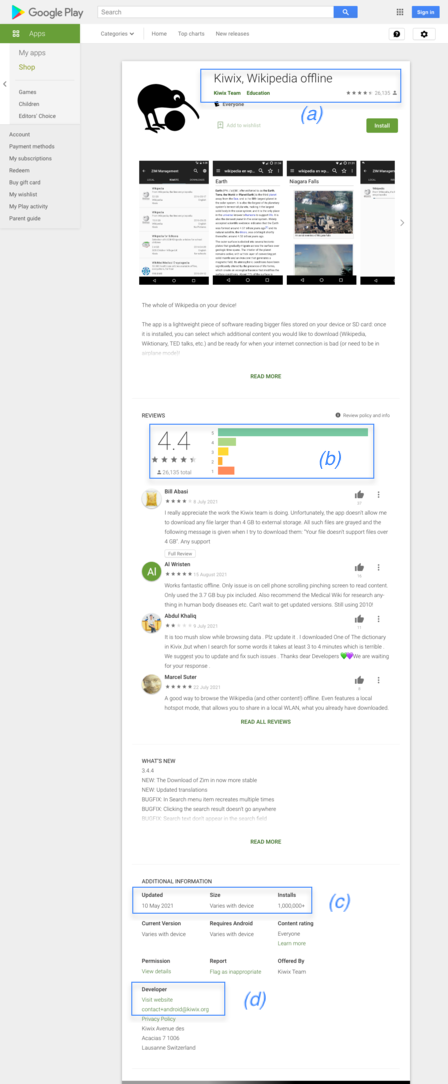
\includegraphics[width=0.42\textwidth]{images/google-play/annotated-resized40pct-2021-09-30-kiwix-app-on-google.png}
  \end{center}
  \caption{Kiwix: app presented in Google Play Store}
  \label{fig:gp-kiwix-app}
\end{wrapfigure}

The projects and their respective organisation need to develop mobile apps and be willing to have mobile analytics for their apps. For the case studies in this research every project included at least one actively used Android app in Google Play\footnote{By having an active app in Google Play they will also have access to the Google Play Console with its dashboard, Android Vitals, release tools, and other related reports. Therefore they will \emph{de-facto} have at least one source of analytics, collected by the Google Android platform.}, however the methodology may work with minor variations for other app stores and mobile platforms.


Various forms of exploration are available. For apps in major app stores the app store may provide pertinent information that can be used to preliminarily select target apps. Figure~\ref{fig:gp-kiwix-app} is how the Kiwix Android app appears to visitors to Google Play when using a web browser (Firefox in this example). Four areas of pertinent information have been highlighted:

\begin{enumerate}[label=(\alph*)]
    \itemsep0em
    \item The category of the app and the count of ratings. The category helps group case studies by category, and also helps compare a particular app with the median crash and ANR rates for apps in that category. More details on these are available in \secref{section-peer-categories}.
    \item More details of the distribution of the ratings.
    \item When the app was last updated in the app store and the number of installs of all versions of this app.
    \item Contact details for the developer~\footnote{That said, like many relationships, a warm lead is more likely to elicit a response than a cold email to the published email address. For this research all bar one of the case studies was established through a warm lead, someone who knows me. The exception was the \href{https://github.com/Phantast/smartnavi}{Smartnavi} project where the connection was established through email.}.
\end{enumerate}

\clearpage
\subsection{Engagement}
The engagement phase includes discussions to determine whether the project team (and their organisation) and the researcher(s) would be willing to participate in a viable and productive case study. It is also a suitable time to agree on the depth, scope, range, and duration of the case study. Similarly concerns and constraints need to be determined and agreed that protect all the stakeholders involved while also allowing the research to be not deliberately biased by the project team/organisation. The stakeholders may extend beyond the primary participants, for instance the end users could potentially be stakeholders in what happens during the case study.

There may also need to be discussion, joint understanding, and agreement on: intellectual property rights, copyright, confidentiality, non disclosure agreements, and so on~\footnote{Note: some researchers may be introduced to these together with the ethical aspects under the term LSEPI, discussed in ~\citet{brooke2018__becoming_professional_a_university_perspective}}. Researchers may be subject to their contract with their institution, employer, and so on. The project team and organisation sometimes may be concerned about any intellectual claims by the researcher's organisation. For the research covered in this thesis copyright is retained by the researcher.

As \citet[p.324]{barroca_2018_bridging_the_gap} notes, timeliness and relevance are vital to industry partners, while they also want to guard against the research being too intrusive or too demanding of their time or other resources. Therefore the research needs to offer something of sufficient relevance and timeliness to the project team and their organisation. 

The ROI of empirical research was discussed and published a relatively long time ago from the perspective of scientific and industrial views~\citet[pp54-57]{prechelt_2007_optimizing_ROI_for_empirical_SE_studies}. Investment in case studies includes dealing with the researcher and their demands so if the researcher is able to use mobile analytics tools, analyse the reports, and investigate initial findings they may reduce the burden placed on the project team and their organisation.

Fortunately research into using mobile analytics to improve the quality of their mobile apps has often provided relevant and timely contributions to the projects, particularly in the more in-depth case studies. Also the projects generally already have at least one form of mobile analytics so the incremental cost is low in terms of tooling.
 
\subsection{The active case study}
If the researcher has direct access to the mobile analytics and/or other materials (such as source code, issue tracking) they can perform at least some of the research directly. If the engagement also includes contributions to the project's materials similarly the researcher may be able to contribute directly if they have write access and/or the facility to fork the codebase and create pull requests. Otherwise the route to mobile analytics reports and any other material available is indirect, via someone who is part of the project and collaborating in the case study. All the case studies included elements of working with and through at least one member of the project team.

For the in-depth case studies where the researcher is more actively involved with the project, the research is likely to have opportunities to work with a variety of team members, and they are also more likely to have direct access to mobile analytics and at least some of the resources. Notes made during and immediately after interviews help to record what was discussed, together with any agreements, actions, or outcomes pertinent to the research and/or the project. Subsequent checking and confirmation of the discussion, for instance in a summary email to the other people in the discussion, 

\citet[p.250]{falessi2010_applying_ESE_to_sw_architecture_etc} states \emph{``there is now a growing need to systematically gather empirical evidence about the advantages or otherwise of tools and methods rather than just rely on promotional anecdotes or rhetoric."}. That was published in 2010, similarly in current times over a decade later, there is a similar growing need to gather evidence about the use of mobile analytics.

In terms of the methodology, during the active case study it is vital to collect and perform ongoing analysis of mobile analytics and whatever other materials are available. Many of these are ephemeral in nature. for instance graphs may change by the minute. There is seldom a manual for the mobile analytics outputs (\textit{e.g.} the reports), furthermore many of the reports are dependent on the underlying data and/or on changes in the underlying service, therefore the researcher often needs to iteratively learn the mobile analytics reporting in an exploratory manner. 

Third-party mobile analytics (including those provided by Google) have terms of use. These terms of use have various names, such as a policy, \textit{e.g.} for Google Play ~\citet{google_play_developer_policy_center}. These may place limitations on data collection and use of the relevant service. For the research covered in this thesis a conservative approach was used in terms of data collection to reduce the risk of consequential issues for the researcher, the project, and the stakeholders for the app. This topic and the implications are expanded on in the \secref{chapter-discussion} chapter.

The choice of tools, including the humble web browser used by the researcher, affects aspects of the ease of collection of on line reports. As an example, the screenshot capability of the Mozilla Firefox browser~\footnote{Described in \url{https://screenshots.firefox.com/}} is far richer than that provided by Google Chrome at the time of writing. Many of the reports in mobile analytics tools require extensive vertical scrolling, Firefox can capture the entire contents easily, Chrome does not. 

Similarly some content is only generated on screen on demand, in response to user actions, for example through scrolling vertically and/or paging through reports. Others are contextual and may only appear when the relevant conditions occur~\footnote{For example, the release management reports in Google Play Console appear for the first 7 days of a new release.}. Therefore, to capture the content the researcher (or their human/automated proxy) needs to perform these actions to obtain these contents and pertinent materials saved/safeguarded to facilitate longer term analysis and provide/record evidence. Note: it is not always practical or useful to record ``everything"; how much is suitable is a topic for future research. Where practical aim to collect the underlying text in addition to visual content; the text can then be processed relatively easily and without needing to be re-keyed.



%%%%% Revised ad-hoc notes during a recent call with Arosha
% Some features are contextual...
% Aim to clearly separate the active analysis vs. the post-hoc stuff for reflective analysis especially across the case studies. Arosha expects most of the research to be based on the post-hoc aspects.

From a research perspective some analysis and verification is likely to occur during the active case study period, and some happens afterwards - based on \emph{post-hoc} analysis. \textbf{MUST-DO Expand on}: Continuous, ongoing, low latency, iterative analysis, verification, course correction, efficacious communications. 

\subsection{\emph{Post-hoc} analysis}
By this stage, the active case study has finished, although in some cases additional updates may be available, for instance if there is ongoing access to mobile analytics as some projects have provided in this research and/or updates from the project team. Nonetheless, for the most part the evidence has been harvested and any active interventions have generally ceased. The time has come to perform \emph{post-hoc} analysis and verify the findings and analysis with the project team wherever practical to do so. 

\textbf{Post-hoc analysis is more research oriented, analysis the active case study is often more project oriented.} 

The nature of the active case studies where there is a need to deal effectively with ephemeral events, data, actions, \textit{etc.} on an opportunistic, often sporadic, basis biases towards tactical findings and outcomes. From a research perspective the active case study may appear messy, chaotic, and yet incomplete. 
The \textit{post-hoc} stage provides the opportunity for complementary more reflective, objective, and strategic research. It can help reduce inadvertent bias in the more immediate tactical work by seeking contraindications, alternatives, and/or mistakes and flaws.

\newthought{Establishing patterns of case studies}~\footnote{\julian{c.f. blood group types O positive, O negative, and their sometimes uni-directional ability to be substituted, etc.}}

This stage may identify patterns within and across one or more case studies. Doing so may help to generalise the research, it may also indicate gaps in the research to date and therefore opportunities to prioritise research aimed at addressing the gaps.
% X-ref to the six perspectives and the findings. What are the data sources that helped me understand the 3 status quo's and the 3 areas or improvement.
In Figure~\ref{fig:six-perspectives} six perspectives are illustrated; these perspectives may help to categorise and group various findings in the \textit{post-hoc} analysis. 

The conclusions, together with their supporting findings and their respective sources, are well worth verifying with the project team wherever practical to do so. Doing so may help protect the integrity of the work and results; it may also provide additional value for the project and the project team. 

\begin{comment}


The \emph{post-hoc} analysis is of material that has been collected, the raw evidence for the research findings. It includes any records and results, identifying patterns in and across case studies, and so on. 

\begin{itemize}
    \itemsep0em
    \item Collating similar failures: 
    \item Bug identification and localisation: Establishing potentially pertinent patterns in the reports, and characterising when a failure \emph{does and does not} occur are part of this work. Obtaining an identifying definitive boundaries may be impractical, the work is often iterative and exploratory in nature and lossy. 
    \item Ordering and ranking clusters of failures:
    \item Bug investigation:
    \item The triage process: 
    \item Comparing information sources:
    \item ...
\end{itemize}

\end{comment}


\subsection{Wrap-up}
The research will need to be wrapped up once the bulk of the research has been completed. (A possible exception is when a case study is ongoing and has no end-date.). The wrap-up can include various actions such as safeguarding and archiving evidence, unsubscribing from services provided for a given case study, publishing what is appropriate to publish in terms of evidence, and so on.

Consider redacting personal details from communications with the stakeholders; for instance, in order to provide emails as supporting evidence for quotes and/or claims made in the research. 

This stage may also provide an opportune period for retrospectives of the case study \textit{and} for the research methods and outcomes, while the case study is still topical. The outputs of the retrospective in some cases may be valuable to fellow researchers, for instance \emph{caveats} for those who follow. 

\subsection{Publication}
Given the practical and empirical nature of the research publishing for industry \emph{and} for academia can help to increase the value of the research. These audiences may have almost orthogonal needs and expectations, for instance industry is particularly interested in highly actionable findings they can apply and obtain productive improvements almost immediately, whereas publication for academia seeks rigour and prefers peer-reviewed acceptance of the material being published.

\section{Rationale}
\newthought{Rationale for the choice of methods}

\newthought{How the methods fit in a framework of theories and complement each other}
\isabel{I would say that the methodology is a description not only of the methods, but also of the rationale for the choice of methods and also how they fit together in a framework of theories, and how they complement and add to each other to provide triangulation and to mitigate threats to validity. So quite a lot to do here.}

\hrulefill
\section{Sources}
\emph{These are interim notes and unlikely to be part of the final version of this chapter.}

\subsection{On Methodology}
\begin{itemize}
    \item \emph{``A Student's Guide to Methodology"}~\citep{clough2012_students_guide_to_methodology}.
    \item \emph{``Creating a wider audience for action research: Learning from case-study research"}~\citep{blichfeldt2006creating}. Online edition available at~\url{http://jrp.icaap.org/index.php/jrp/article/view/23/43}.
    \item \emph{``Action research or case study?"} \url{https://www.nicole-brown.co.uk/action-research-or-case-study/}
    \item \emph{``A gentle guide to research methods"}~\citep{rugg2006_gentle_guide_to_research_methods}.
    \item \emph{``Stepping Stones to Achieving your Doctorate"}~\citep{trafford2008_stepping_stones_to_achieving_your_doctorate}.
    \item \emph{``The How To of Qualitative Research: Strategies for Executing High Quality Projects"}~\citep{aurini2016_how_to_of_qualitative_research}.
    \item \emph{``Empirical Research Methods in Software Engineering"}~\citep{Wohlin2003_empirical_research_methods_in_software_engineering} \textbf{This is one of the key papers to provide support and evidence for using empirical research methods in my research.}
    \item \emph{``Evaluation and Measurement of Software Process Improvement—A Systematic Literature Review"}~\citep{unterkalmsteiner2012_evaluation_and_measurement_of_spi_a_slr}
    \begin{itemize}
        \item ``evaluation strategies were identified, wherein the most common one, “Pre-Post Comparison,” was applied in 49 percent of the inspected papers. Quality was the most measured attribute (62 percent)"
        \item ``CONCLUSION-The evaluation validity of SPI initiatives is challenged by the scarce consideration of potential confounding factors, particularly given that “Pre-Post Comparison” was identified as the most common evaluation strategy, and the inaccurate descriptions of the evaluation context. Measurements to assess the short and mid-term impact of SPI initiatives prevail, whereas long-term measurements in terms of customer satisfaction and return on investment tend to be less used."
    \end{itemize}
    \item \emph{``Grounded theory in software engineering research: a critical review and guidelines"} \url{https://doi.org/10.1145/2884781.2884833} if I decide to wade into grounded theory... (I aim not to).
\end{itemize}

\isabel{Next call, 2 hours on Thursday 9th Sept 09:30 - 11:30 - Whiteboarding session.}

\section{Placeholders}
\begin{itemize}
    \item \citep{soiferman2010_compare_and_contrast_inductive_and_deductive_research_approaches}
\end{itemize}
